\subsection{COMPLEXIFICATION OF A FINITE-DIMENSIONAL REAL LIE GROUP}

Lemma 7. Let B be a group, A a normal subgroup of B, C the group B/A and i: A → B and p: B → C the canonical morphisms. Let A' be a group and f a homomorphism of A into A'. Let ω be a morphism of B into the automorphism group of A'. Suppose that, for \(a \in A'\) , \(a' \in A'\) , \(b \in B\) ,

\[
f (b a b ^ {- 1}) = \omega (b) f (a), \quad \omega (a) a ^ {\prime} = f (a) a ^ {\prime} f (a) ^ {- 1}.
\]

Let \(\mathbf{B}''\) be the semi-direct product of \(\mathbf{B}\) by \(\mathbf{A}'\) relative to \(\omega\) and \(q\) the canonical morphism of \(\mathbf{B}''\) onto \(\mathbf{B}\) .

\begin{enumerate}
\def\labelenumi{(\roman{enumi})}
\item
  The mapping \(a \mapsto (f(a^{-1}), i(a))\) of A into B'' is a morphism of A onto a normal subgroup D of B''. Let B' = B''/D and \(i' \colon A' \to B'\) , \(g \colon B \to B'\) be the morphisms of A' and B into B' derived when taking quotients from the canonical injections of A' and B into B''.
\item
  The morphism \(p \circ q\) of \(\mathbf{B}''\) into \(\mathbf{C}\) defines when passing to the quotient a morphism of \(\mathbf{B}'\) into \(\mathbf{C}\) .
\item
  \(i'\) is injective, \(p'\) is surjective, \(\operatorname{Ker}(p') = \operatorname{Im}(i')\) and the following diagram is commutative
\end{enumerate}

\begin{enumerate}
\def\labelenumi{(\arabic{enumi})}
\setcounter{enumi}{3}
\tightlist
\item
\end{enumerate}

\pandocbounded{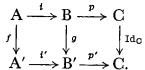
\includegraphics[keepaspectratio]{images/part002_08e8b4be.jpg}}

\begin{enumerate}
\def\labelenumi{(\roman{enumi})}
\setcounter{enumi}{3}
\tightlist
\item
  If \(b \in \mathbf{B}\) and \(a' \in \mathbf{A}'\) , then
\end{enumerate}

\[
g (b) i ^ {\prime} \left(a ^ {\prime}\right) g (b) ^ {- 1} = i ^ {\prime} (\omega (b) a ^ {\prime}).
\]

\begin{enumerate}
\def\labelenumi{(\roman{enumi})}
\tightlist
\item
  For \(a_{1}\) , \(a_{2}\) in A, we have, in B'',
\end{enumerate}

\[
\begin{array}{r l} (f (a _ {1} ^ {- 1}), i (a _ {1})) (f (a _ {2} ^ {- 1}), i (a _ {2})) & = (f (a _ {1} ^ {- 1}) (\omega (a _ {1}) f (a _ {2} ^ {- 1})), i (a _ {1}) i (a _ {2})) \\ & = (f (a _ {1} ^ {- 1}) f (a _ {1} a _ {2} ^ {- 1} a _ {1} ^ {- 1}), i (a _ {1} a _ {2})) \\ & = (f ((a _ {1} a _ {2}) ^ {- 1}, i (a _ {1} a _ {2})) \end{array}
\]

and hence \(a \mapsto (f(a^{-1}), i(a))\) is a homomorphism \(h\) of \(A\) into \(B''\) . Let \(a \in A\) , \(a' \in A'\) , \(b \in B\) ; then, in \(B''\) ,

\[
\begin{array}{r l} b h (a) b ^ {- 1} & = b f (a ^ {- 1}) a b ^ {- 1} = (\omega (b) f (a ^ {- 1})) (b a b ^ {- 1}) \\ & = f (b a ^ {- 1} b ^ {- 1}) (b a b ^ {- 1}) = h (b a b ^ {- 1}) \\ a ^ {\prime} h (a) a ^ {\prime - 1} & = a ^ {\prime} f (a ^ {- 1}) a a ^ {\prime - 1} = a ^ {\prime} f (a ^ {- 1}) (\omega (a) a ^ {\prime - 1}) a \\ & = a ^ {\prime} f (a ^ {- 1}) f (a) a ^ {\prime - 1} f (a ^ {- 1}) a = h (a) \end{array}
\]

and hence \(h(A) = D\) is normal in \(B''\) .

\begin{enumerate}
\def\labelenumi{(\roman{enumi})}
\setcounter{enumi}{1}
\tightlist
\item
  For \(a \in A\) ,
\end{enumerate}

\[
(p \circ q) (h (a)) = p (q (f (a ^ {- 1}) a)) = p (a) = e
\]

and hence \(p \circ q\) is trivial on D.

\begin{enumerate}
\def\labelenumi{(\roman{enumi})}
\setcounter{enumi}{2}
\tightlist
\item
  Let \(a' \in A'\) be such that \(i'(a') = e\) ; then \(a' \in D\) and hence there exists \(a \in A\) such that \(a' = f(a^{-1})a\) ; this implies \(a = e\) , whence \(a' = e\) ; thus \(i'\) is injective. As \(p\) and \(q\) are surjective, \(p'\) is surjective.
\end{enumerate}

Let \(r\) denote the canonical morphism of \(B''\) onto \(B'\) . Let \(a' \in A'\) , \(b \in B\) and \(b' = r(a'b)\) . If \(b' \in \operatorname{Im}(i')\) , there exists \(a_1' \in A'\) such that \(b' = r(a_1')\) ; then there exists \(a \in A\) such that \(a'b = a_1'f(a^{-1})a\) , whence \(b = a \in A\) and

\[
p ^ {\prime} (b ^ {\prime}) = p (q (a ^ {\prime} b)) = p (b) = e;
\]

thus, \(\operatorname{Im}(i') \subset \operatorname{Ker}(p')\) . We preserve the notation \(a', b, b'\) but assume that \(b' \in \operatorname{Ker}(p')\) ; then \(e = p'(b') = p(q(a'b)) = p(b)\) and hence \(b \in A\) , whence

\[
b ^ {\prime} = r (a ^ {\prime} f (b) f (b ^ {- 1}) b) = r (a ^ {\prime} f (b)) \in \operatorname{Im} (i ^ {\prime});
\]

thus \(\operatorname{Ker}(p') \subset \operatorname{Im}(i')\) .

If \(a\in \mathbf{A}\) , then

\[
i ^ {\prime} (f (a)) = r (f (a)) = r (f (a) f \left(a ^ {- 1}\right) a) = r (a) = g (i (a)).
\]

If \(b\in \mathbf{B}\) , then

\[
p ^ {\prime} (g (b)) = p (b)
\]

and hence diagram (4) is commutative.

\begin{enumerate}
\def\labelenumi{(\roman{enumi})}
\setcounter{enumi}{3}
\tightlist
\item
  Let \(b \in \mathbf{B}\) , \(a' \in \mathbf{A}'\) . Then
\end{enumerate}

\[
\begin{array}{r} g (b) i ^ {\prime} (a ^ {\prime}) g (b) ^ {- 1} = r (b) r (a ^ {\prime}) r (b) ^ {- 1} = r (b a ^ {\prime} b ^ {- 1}) \\ = r (\omega (b) a ^ {\prime}) = i ^ {\prime} (\omega (b) a ^ {\prime}). \end{array}
\]

PROPOSITION 20. Let G be a finite-dimensional real Lie group.

\begin{enumerate}
\def\labelenumi{(\roman{enumi})}
\item
  There exist a complex Lie group \(\tilde{\mathbf{G}}\) and an \(\mathbf{R}\) -analytic morphism \(\gamma\) of \(\mathbf{G}\) into \(\tilde{\mathbf{G}}\) with the following properties: for every complex Lie group \(\mathbf{H}\) and every \(\mathbf{R}\) -analytic morphism \(\phi\) of \(\mathbf{G}\) into \(\mathbf{H}\) , there exists one and only one \(\mathbf{C}\) -analytic morphism \(\psi\) of \(\tilde{\mathbf{G}}\) into \(\mathbf{H}\) such that \(\phi = \psi \circ \gamma\) .
\item
  If \((\tilde{\mathbf{G}}', \gamma')\) has the same properties as \((\tilde{\mathbf{G}}, \gamma)\) , there exists one and only one isomorphism \(\theta\) of \(\tilde{\mathbf{G}}\) onto \(\tilde{\mathbf{G}}'\) such that \(\theta \circ \gamma = \gamma'\) .
\item
  The \(\mathbf{C}\) -linear mapping of \(\mathrm{L}(\mathrm{G}) \otimes \mathbf{C}\) into \(\mathrm{L}(\tilde{\mathrm{G}})\) which extends \(\mathrm{L}(\gamma)\) is surjective; in particular \(\dim_{\mathbf{C}}(\tilde{\mathbf{G}}) \leqslant \dim_{\mathbf{R}}(\mathrm{G})\) .
\end{enumerate}

Assertion (ii) is obvious. We prove the existence of an ordered pair \((\tilde{G},\gamma)\) with properties (i) and (iii).

\begin{enumerate}
\def\labelenumi{(\alph{enumi})}
\tightlist
\item
  Suppose first that \(G\) is connected. Let \(g = L(G)\) , \(g_{\mathbf{C}} = g \otimes_{\mathbf{R}} \mathbf{C}\) be the complexification of \(g\) , \(S\) (resp. \(S'\) ) the simply connected real (resp. complex) Lie group with Lie algebra \(g\) (resp. \(g_{\mathbf{C}}\) ) and \(\sigma\) the unique \(\mathbf{R}\) -analytic morphism of \(S\) into \(S'\) such that \(L(\sigma)\) is the canonical injection of \(g\) into \(g_{\mathbf{C}}\) . Let \(\pi\) be the unique \(\mathbf{R}\) -analytic morphism of \(S\) onto \(G\) such that \(L(\pi) = I d_{L(G)}\) and \(F = K e r \pi\) .
\end{enumerate}

\pandocbounded{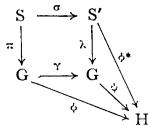
\includegraphics[keepaspectratio]{images/part002_6429af2f.jpg}}

For every complex Lie group H and every R-analytic morphism \(\phi\) of G into H, \(L(\phi): g \to L(H)\) has a unique C-linear extension to \(g_{C}\) and this extension is of the form \(L(\phi^{*})\) , where \(\phi^{*}\) is a C-analytic morphism of \(S'\) into H. Then

\[
\mathrm{L} (\phi \circ \pi) = \mathrm{L} (\phi) \circ \mathrm{L} (\pi) = \mathrm{L} (\phi) = \mathrm{L} (\phi^ {*}) \circ \mathrm{L} (\sigma) = \mathrm{L} (\phi^ {*} \circ \sigma)
\]

and hence \(\phi \circ \pi = \phi^{*} \circ \sigma\) . Therefore \(\phi^{*}(\sigma(F)) = \phi(\pi(F)) = \{e\}\) , whence

\[
\sigma (\mathrm{F}) \subset \operatorname{Ker} \phi^ {*}.
\]

Let P be the intersection of the Ker \(\phi^{*}\) for variable \(\phi\) . This is a normal Lie subgroup of \(S'\) (no. 2, Corollary 3 to Proposition 1). Let \(\tilde{G} = S'/P\) and \(\lambda: \mathbf{S}' \to \tilde{\mathbf{G}}\) be the canonical morphism. Then \(\sigma(\mathbf{F}) \subset \mathbf{P}\) and hence there exists one and only one \(\mathbf{R}\) -analytic morphism \(\gamma\) of \(\mathbf{G}\) into \(\tilde{\mathbf{G}}\) such that \(\gamma \circ \pi = \lambda \circ \sigma\) . If \(\psi: \tilde{\mathbf{G}} \to \mathbf{H}\) denotes the morphism derived from \(\phi^*\) when passing to the quotient, then

\[
(\phi \circ \gamma) \circ \pi = \psi \circ (\lambda \circ \sigma) = \phi^ {*} \circ \sigma = \phi \circ \pi
\]

whence \(\psi \circ \gamma = \phi\) . Clearly \(\mathrm{L}(\psi)\) , and hence \(\psi\) , are determined uniquely by the equality \(\psi \circ \gamma = \phi\) . Thus we have proved that the ordered pair \((\tilde{G}, \gamma)\) has properties (i) and (iii).

\begin{enumerate}
\def\labelenumi{(\alph{enumi})}
\setcounter{enumi}{1}
\tightlist
\item
  We pass now to the general case. Let \(\mathbf{F}\) be the identity component of \(\mathrm{G},\mathrm{M} = \mathrm{G} / \mathrm{F}\) and \(i\colon \mathrm{F}\to \mathrm{G}\) and \(p\colon \mathrm{G}\rightarrow \mathrm{M}\) be the canonical morphisms. We apply part (a) of the proof to F. We obtain an ordered pair \((\tilde{\mathbf{F}},\delta)\) . For all \(g\in \mathrm{G}\) , Int \(g|\mathrm{F} = \omega '(g)\) is an automorphism of F. By the universal property of \(\tilde{\mathbf{F}}\) , there exists one and only one automorphism \(\omega (g)\) of the complex Lie group \(\tilde{\mathbf{F}}\) such that \(\delta \circ \omega '(g) = \omega (g)\circ \delta\) . Clearly \(\omega\) is a morphism of G into \(\operatorname {Aut}(\tilde{\mathbf{F}})\) . If \(g\in \mathbf{G}\) and \(f\in \tilde{\mathbf{F}}\) , then
\end{enumerate}

\[
\delta (g f g ^ {- 1}) = (\delta \circ \omega^ {\prime} (g)) (f) = (\omega (g) \circ \delta) (f) = \omega (g) (\delta (f)).
\]

If \(f \in \mathbf{F}\) , then \(\delta \circ (\operatorname{Int}_{\mathbb{F}} f) = (\operatorname{Int}_{\tilde{\mathbb{F}}} \delta(f)) \circ \delta\) and \(\operatorname{Int}_{\tilde{\mathbb{F}}} \delta(f)\) is an automorphism of the complex Lie group \(\tilde{\mathbf{F}}\) ; hence \(\operatorname{Int}_{\tilde{\mathbb{F}}} \delta(f) = \omega(f)\) .

Hence Lemma 7 can be applied, which gives a diagram

\[
\begin{array}{c} \mathrm{F} \xrightarrow {i} \mathrm{G} \xrightarrow {p} \mathrm{M} \\ \delta \Big \downarrow \qquad \qquad \qquad \gamma \Big \downarrow \qquad \qquad \Big \downarrow \mathrm{Id} \\ \tilde {\mathrm{F}} \xrightarrow {\tilde {i}} \tilde {\mathrm{G}} \xrightarrow {\tilde {p}} \mathrm{M}. \end{array}
\]

Let \(\tilde{\mathbf{F}}\) be identified with a normal subgroup of \(\tilde{\mathbf{G}}\) by means of \(\tilde{i}\) . The group \(\tilde{\mathbf{G}}\) is generated by \(\tilde{\mathbf{F}}\) and \(\gamma (\mathbf{G})\) ; hence the automorphisms of \(\tilde{\mathbf{F}}\) defined by the elements of \(\tilde{\mathbf{G}}\) are automorphisms of the complex Lie group structure. By § 1, no. 9, Proposition 18, there exists one and only one complex Lie group structure on \(\tilde{\mathbf{G}}\) such that \(\tilde{\mathbf{F}}\) is an open Lie subgroup of \(\tilde{\mathbf{G}}\) . Henceforth \(\tilde{\mathbf{G}}\) will have this structure. As \(\delta\) is \(\mathbf{R}\) -analytic, \(\gamma\) is \(\mathbf{R}\) -analytic.

The ordered pair \((\tilde{G},\gamma)\) has property (iii) of the proposition. We show that it has property (i). Let H be a complex Lie group and \(\phi\) an R-analytic morphism of G into H. There exists a C-analytic morphism \(\eta\) of \(\tilde{F}\) into H such that \(\eta \circ \delta = \phi |F\) . Let \(g\in G\) . The mappings

\[
f \mapsto \eta (\omega (g) f), \quad f \mapsto \phi (g) \eta (f) \phi (g) ^ {- 1}
\]

of \(\tilde{\mathbf{F}}\) into \(\mathbf{H}\) are \(\mathbf{C}\) -analytic morphisms; they coincide on \(\delta(\mathbf{F})\) , for, if \(f' \in \mathbf{F}\) , then

\[
\begin{array}{r} \phi (g) \eta (\delta (f ^ {\prime})) \phi (g) ^ {- 1} = \phi (g) \phi (f ^ {\prime}) \phi (g) ^ {- 1} = \phi (g f ^ {\prime} g ^ {- 1}) \\ = \eta (\delta (g f ^ {\prime} g ^ {- 1})) = \eta (\omega (g) \delta (f ^ {\prime})); \end{array}
\]

therefore \(\eta (\omega (g)f) = \phi (g)\eta (f)\phi (g)^{-1}\) for all \(g\in G\) and all \(f\in \tilde{\mathbf{F}}\) . If \(\mathbf{G}'\) denotes the semi-direct product of \(\mathbf{G}\) by \(\tilde{\mathbf{F}}\) relative to \(\omega\) , there then exists a morphism \(\zeta\) of the group \(\mathbf{G}'\) into \(\mathrm{H}\) which coincides with \(\phi\) on \(\mathrm{G}\) and with \(\eta\) on \(\tilde{\mathbf{F}}\) . For \(f\in \mathbf{F}\) ,

\[
\zeta (\delta (f ^ {- 1}) f) = \eta (\delta (f ^ {- 1})) \phi (f) = \phi (f ^ {- 1}) \phi (f) = e.
\]

Hence \(\zeta\) defines on passing to the quotient a morphism \(\psi\) of \(\tilde{\mathbf{G}}\) into H. Then \(\psi \circ \gamma = \phi\) and \(\psi \circ \tilde{i} = \eta\) ; the latter equality implies that \(\psi\) is C-analytic.

Finally, let \(\psi'\) be a \(\mathbf{C}\) -analytic morphism of \(\tilde{\mathbf{G}}\) into \(\mathbf{H}\) such that \(\phi = \psi' \circ \gamma\) . Then

\[
\psi^ {\prime} \circ \tilde {i} \circ \delta = \psi^ {\prime} \circ \gamma \circ i = \phi \circ i = \psi \circ \tilde {i} \circ \delta
\]

and hence \(\psi' \circ \tilde{i} = \psi \circ \tilde{i}\) . As \(\tilde{G}\) is generated by \(\tilde{i}(\tilde{\mathrm{F}})\) and \(\gamma(G)\) , \(\psi' = \psi\) .

DEFINITION 4. \((\tilde{G},\gamma)\), or simply \(\tilde{G}\) , is called the universal complexification of G.

Remarks. (1) Let \((\tilde{\mathbf{G}},\gamma)\) be the universal complexification of G. Let \(G_0\) (resp. \(\tilde{G}_0\) ) be the identity component of G (resp. \(\tilde{G}\) ). By the proof of Proposition 20, \((\tilde{G}_0,\gamma |G_0)\) is the universal complexification of \(G_0\) and the composite morphism

\[
\mathrm{G} \rightarrow \tilde {\mathrm{G}} \rightarrow \tilde {\mathrm{G}} / \tilde {\mathrm{G}} _ {0}
\]

defines on passing to the quotient an isomorphism of \(\mathbf{G} / \mathbf{G}_0\) onto \(\tilde{\mathbf{G}} / \tilde{\mathbf{G}}_0\) .

\begin{enumerate}
\def\labelenumi{(\arabic{enumi})}
\setcounter{enumi}{1}
\tightlist
\item
  Suppose that G is simply connected. Let \(g = L(G)\) , \(g_{c}\) be the complexification of g, \(S'\) the simply connected complex Lie group with Lie algebra \(g_{c}\) and \(\sigma\) the morphism of G into \(S'\) such that \(L(\sigma)\) is the canonical injection of g into \(g_{c}\) . We again use the notation of the proof of Proposition 20, part (a). If \(H = S'\) and \(\phi = \sigma\) , then \(\phi^{*} = I d_{g}\) . Hence \((S', \sigma)\) is the universal complexification of G. Note that \(\sigma\) is not in general injective (Exercise 16); however its kernel is discrete since \(L(\sigma)\) is injective. On the other hand, let \(\theta\) be the involution of \(g_{c}\) defined by g and let \(\eta\) be the corresponding automorphism of the underlying real Lie group of \(S'\) ; let \(S'^{\eta}\) be the set of points of \(S'\) invariant under \(\eta\) ; it is a real Lie subgroup of \(S'\) with Lie algebra g (§3, no. 8, Corollary 1 to Proposition 29). By no. 1, Corollary 1 to Proposition 1, \(\sigma(G)\) is a real integral subgroup of \(S'\) with Lie algebra g and hence \(\sigma(G)\) is the identity component of \(S'^{\eta}\) ; in particular \(\sigma(G)\) is a real Lie subgroup of \(S'\) .
\end{enumerate}

